% Co-governed and enforced under the Sovereign Integrity Protocol License (SIP License v1.1):
% https://github.com/tensorrent/ACS-Framework/blob/main/LICENSE
\documentclass[11pt,a4paper]{article}

%% ═══════════════════════════════════════════════════════════════════════════
%% VISUAL STYLE — ACS Trilogy, presentation-grade typography
%% ═══════════════════════════════════════════════════════════════════════════
\usepackage[T1]{fontenc}
\usepackage{amsmath,amssymb,amsthm}
\usepackage{geometry}
\usepackage{xcolor}
\usepackage{graphicx}
\graphicspath{{figures/}}
\usepackage{enumitem}
\usepackage{booktabs}
\usepackage[expansion=false]{microtype}
\usepackage[numbers,sort&compress]{natbib}
\usepackage{mathtools}
\usepackage{fancyhdr}
\usepackage{titlesec}
\usepackage{needspace}
\usepackage{placeins}
\usepackage{etoolbox}
\usepackage{tocloft}

\definecolor{acsprimary}{HTML}{1a237e}
\definecolor{acssecondary}{HTML}{3949ab}
\definecolor{acsaccent}{HTML}{c62828}
\definecolor{acsgold}{HTML}{b8860b}
\definecolor{acsgreen}{HTML}{2e7d32}
\definecolor{acsslate}{HTML}{37474f}
\definecolor{acslight}{HTML}{e8eaf6}
\definecolor{acsrule}{HTML}{9fa8da}

\usepackage[labelfont={bf,small,color=acsprimary!90!black},
            textfont={small,it}]{caption}
\usepackage{hyperref}
\usepackage{xurl}
\usepackage{bookmark}
\setlength{\emergencystretch}{2em}

\geometry{top=1.15in,bottom=1.15in,left=1.2in,right=1.2in,
          headheight=16pt,headsep=0.25in,footskip=0.45in}

\hypersetup{colorlinks=true,linkcolor=acsprimary,citecolor=acssecondary,
            urlcolor=acsaccent,pdfpagemode=UseOutlines,bookmarksopen=true,pageanchor=false}

\pagestyle{fancy}
\fancyhf{}
\renewcommand{\headrulewidth}{0.4pt}
\renewcommand{\footrulewidth}{0pt}
\fancyheadoffset{0pt}
\fancyhead[L]{\small\color{acsslate}\itshape\leftmark}
\fancyhead[R]{\small\color{acsslate}\textit{Riemann Spectral ACS}}
\fancyfoot[C]{\small\color{acsslate}\thepage}
\renewcommand{\sectionmark}[1]{\markboth{\S\thesection.\ #1}{}}

\titleformat{\section}{\normalfont\Large\bfseries\color{acsprimary}}
  {\thesection}{0.7em}{}[\vspace{-2pt}{\color{acsrule}\rule{\textwidth}{0.4pt}}]
\titleformat{\subsection}{\normalfont\large\bfseries\color{acssecondary}}
  {\thesubsection}{0.7em}{}
\titleformat{\subsubsection}{\normalfont\normalsize\bfseries\color{acsslate}}
  {\thesubsubsection}{0.7em}{}
\titlespacing*{\section}{0pt}{2.4ex plus 0.9ex minus 0.4ex}{1.4ex plus 0.3ex}
\titlespacing*{\subsection}{0pt}{2.0ex plus 0.7ex minus 0.3ex}{0.9ex plus 0.2ex}
\titlespacing*{\subsubsection}{0pt}{1.6ex plus 0.5ex minus 0.2ex}{0.7ex}

\theoremstyle{plain}
\newtheorem{theorem}{Theorem}[section]
\newtheorem{lemma}[theorem]{Lemma}
\newtheorem{corollary}[theorem]{Corollary}
\newtheorem{proposition}[theorem]{Proposition}
\theoremstyle{definition}
\newtheorem{definition}[theorem]{Definition}
\theoremstyle{remark}
\newtheorem*{theorem*}{Theorem}
\newtheorem{remark}[theorem]{Remark}
\newtheorem{conjecture}[theorem]{Conjecture}

\setlist[itemize]{leftmargin=1.3em,itemsep=2pt,topsep=3pt,parsep=0pt}
\setlist[enumerate]{leftmargin=1.5em,itemsep=2pt,topsep=3pt,parsep=0pt}
\setcounter{tocdepth}{2}
\setlength{\cftbeforesecskip}{2pt}
\setlength{\cftbeforesubsecskip}{0.5pt}
\widowpenalty=10000
\clubpenalty=10000
\displaywidowpenalty=10000
%

\newcommand{\DI}{\Delta\mathcal{I}}
\newcommand{\TE}{\mathrm{TE}}
\newcommand{\Order}[1]{\mathcal{O}(#1)}
\newcommand{\eps}{\varepsilon}

\title{\textbf{Spectral Susceptibility and Renormalized Stability on the Riemann Critical Line}\\[0.4em]
       \large Transfer Entropy, Stationarity, and an ACS Approach to the Riemann Hypothesis}
\author{Bradley Wallace\\[0.3em]
        \small \textit{Independent Researcher}\\[0.2em]
        \small \texttt{Riemann Spectral ACS}}
\date{March 2026}

% Publication typography: portable paths, bounded tables, paragraph flexibility.
\usepackage{xurl,adjustbox}
\setlength{\emergencystretch}{3em}
\begin{document}

%% ═══════════════════════════════════════════════════════════════════════════
%% CUSTOM TITLE PAGE
%% ═══════════════════════════════════════════════════════════════════════════
\begin{titlepage}
\thispagestyle{empty}

\noindent{\color{acsrule}\rule{\textwidth}{0.4pt}}
\vspace{6pt}
\noindent{\footnotesize\color{acsslate}\hfill\textit{Riemann Spectral ACS} \quad|\quad \textit{Independent Research} \quad|\quad March 2026}
\vspace{6pt}
\noindent{\color{acsrule}\rule{\textwidth}{0.4pt}}

\vspace{0.6in}

\begin{center}
  {\Huge\bfseries\color{acsprimary} The Riemann Spectral ACS}\\[0.4em]
  {\Large\color{acsslate} Stationarity as a Characterisation of the Critical Line}\\[1.2em]
  {\normalsize\itshape\color{acsslate}
    Information Asymmetry, Transfer Entropy, and an ACS Approach to the Riemann Hypothesis}\\[2.0em]
  {\large\bfseries Bradley Wallace}\\[0.25em]
  {\small\itshape\color{acsslate} Independent Researcher}
\end{center}
\par\smallskip\noindent\textbf{Publication status (24 September 2026).}
This version includes a claim-specific amendment at the end of the main text.
That amendment governs earlier physical interpretations and distinguishes
retained calculations from withdrawn or unresolved inferences.\par\smallskip


\vspace{0.5in}

\begin{center}
\begin{minipage}{0.88\textwidth}
\begin{center}
  {\bfseries\color{acsprimary}\large Abstract}\\[0.3em]
  {\color{acsrule}\rule{1.2in}{0.3pt}}
\end{center}
\vspace{0.5em}
\small\noindent
We study finite spectral diagnostics linking prime and zero descriptions of
the Riemann zeta function through the classical explicit formula. Fixed
finite sums built from critical-line coefficients have bounded variance
for arbitrary real input ordinates. A separate elementary theorem detects
active positive real exponents in a finite exponential sum after identical
exponents are combined; it needs no quantitative minimum-gap assumption.
Neither statement identifies the real parts of actual zeta zeros from
their imaginary parts.

Historical calculations report variance diagnostics through $2{,}001{,}052$
supplied ordinates, finite Wronskian tests, prime-power Fourier signatures,
and character-dependent $L$-function signatures. They characterize the
specified observations and model families. Some earlier numerical-to-theorem
inferences are withdrawn: a sampled cross-correlation is not a global
supremum, a fixed finite bound is not an infinite-sum bound, and a
self-adjoint diagonal matrix constructed from real ordinates does not
establish Hilbert--P\'olya identification.

The corrected arithmetic criterion is the classical equivalence between
RH and $\psi(x)-x=O(\sqrt{x}\log^2x)$. In logarithmic coordinates, the
full normalized error is $O(u^2)$ under RH, whereas the canonical code
computes a fixed finite bounded sum. Proving the full bound independently
of RH, or constructing a natural operator with complete spectral
identification $z_\rho=-i(\rho-1/2)$, remains open. The critical line is a
defined one-dimensional locus; a geometric rendering or a proposed
underlying carrier does not change that statement. This revision applies
the existing Frontier corrections and preserves the boundary between
finite evidence, conditional results, and the unsolved RH claim.

\end{minipage}
\end{center}

\vfill

\noindent{\color{acsrule}\rule{\textwidth}{0.4pt}}
\end{titlepage}

\clearpage
\hypersetup{pageanchor=true}
\pagenumbering{roman}
\setcounter{page}{1}
\markboth{Contents}{}
\tableofcontents
\clearpage
\pagenumbering{arabic}
\setcounter{page}{1}

\section*{Scope correction: 22 September 2026}
The September Frontier audit already separated finite sums, full arithmetic
error, and natural-operator identification. This revision incorporates those
corrections into the live text. The former AM--GM non-cancellation argument,
gap-dependent converse, zero-valued stability ratio, exclusive pure-cosine
shear derivative, and constant bound for
the full normalized arithmetic error are withdrawn in their earlier forms.
Finite numerical diagnostics remain historical measurements with their stated
input families; they do not discharge the missing identification or infinite
limit. The source history and dated Frontier snapshots retain the earlier text.
Other physical and information-theoretic identifications in this paper require
their own hypotheses; this scoped revision does not certify them.

For clarity, the critical line is the one-real-dimensional set
$L=\{s:\Re s=1/2\}$. The vertical reflection is
$R(s)=1-\overline{s}$, with $\operatorname{Fix}(R)=L$;
$s\mapsto1-s$ alone fixes only the point $1/2$. A change of coordinates can
bend the image of $L$ without changing its intrinsic dimension. The completed
zeta function's symmetries do not force its zeros to lie on this fixed locus.

\section{The ACS Framework (Summary)}
\label{sec:acs}

\noindent\textit{This section provides a self-contained summary of the ACS
framework.  The full development, including all proofs and the accompanying
verification suite, is in the companion paper~\cite{Wallace2026a}.}

\medskip\noindent
The Asymmetric Codependent System (ACS) is defined in~\cite{Wallace2026a}.
For this paper, the key result is the BCH--TE morphism: the net transfer
entropy $\DI(\eps) = \eps\langle f{-}g, \nabla\log\mu\rangle + 2\eps^2\langle[f,g],\nabla\log\mu\rangle + \Order{\eps^3}$, where $[f,g]$ is the Lie bracket of the ACS flow generators and $\mu$ is the SRB invariant measure.
\section{The Riemann Spectral Function as an ACS}
\label{sec:riemann}
%% ─────────────────────────────────────────────────────────────────────────────

\subsection{The spectral function \texorpdfstring{$F_N(x)$}{F\_N(x)}}

Throughout this section, the prime sequence $\{p_n\}$ and Riemann zero sequence $\{\gamma_k\}$ are equipped with the point-process measures defined in the ACS measure definition~\cite{Wallace2026a} and the accompanying remark.  Transfer entropy is computed with respect to those measures; ergodicity of $\{p_n\}$ follows from the Prime Number Theorem (Vinogradov equidistribution), and $\{\gamma_k\}$ carries the GUE pair-correlation measure (Montgomery--Odlyzko law~\cite{Montgomery1973,Odlyzko1987}).  With this foundation, $\DI$ is well-defined on both sequences.

The prime explicit formula (Riemann--von Mangoldt; see~\cite{Davenport2000} for the classical theory) states:
\begin{equation}
  \psi(x) = x - \sum_\rho \frac{x^\rho}{\rho} - \log(2\pi) - \tfrac{1}{2}\log(1-x^{-2}),
\end{equation}
where the sum runs over non-trivial zeros $\rho = \sigma + i\gamma$ of $\zeta$.
For supplied positive real ordinates, using critical-line coefficients,
define the finite diagnostic below. Its argument is logarithmic: here
$x=\log p$, rather than the arithmetic argument in the preceding formula.
This definition has already fixed the real parts to $1/2$; it is not the
general zero contribution when the real parts are unknown.
\begin{equation}
  F_N(x) = \sum_{k=1}^N A_k \varphi_k(x), 
  \quad A_k = \frac{1}{\tfrac{1}{4}+\gamma_k^2}, 
  \quad \varphi_k(x) = \tfrac{1}{2}\cos(\gamma_k x) + \gamma_k\sin(\gamma_k x),
\end{equation}
evaluated at $x = \ln p$ for primes $p$.

\begin{remark}[Notation: three mode conventions are in use]
\label{rem:phi-conventions}
This paper uses $\varphi_k$ in three distinct normalisations, and the reader
must track which is live, because the same object (notably the Wronskian
$W[\varphi_k,\varphi_j]$) takes numerically very different values under them.
\textbf{(C1)} the \emph{log-argument} form above,
$\varphi_k(x) = \tfrac12\cos(\gamma_k x) + \gamma_k\sin(\gamma_k x)$ with
$x = \ln p$, used in this section and for the stationarity measure.
\textbf{(C2)} the \emph{envelope-stripped} form
$\varphi_k(x) = \cos(\gamma_k \ln x)/\sqrt{x}$, used where the modes are
displayed against $\ln x$.
\textbf{(C3)} the \emph{general-$\sigma$} form
$\varphi_k(t) = e^{\sigma t}\left[\sigma\cos(\gamma_k t) + \gamma_k\sin(\gamma_k t)\right]/(\sigma^2+\gamma_k^2)$,
used in the harmonic-oscillator remark \emph{and in every quoted Wronskian
magnitude}. These are distinct observables or rescalings and must not be
substituted for one another in a boundedness, variance, or growth claim.
A variable-dependent envelope need not cancel in a ratio or a stationarity
statement. The actual normalized full-zero contribution in logarithmic
coordinate $u$ is proportional to $e^{(\rho-1/2)u}/\rho$.

\medskip
\noindent
\textbf{Which convention the Wronskian numbers use.}  The range
$|W| \in [8.6\times10^{-5},\, 0.19]$ quoted below is computed under
\textbf{C3}, in the $t = \ln x$ variable at $t = 1$, $\sigma = 1/2$, over all
$\binom{50}{2} = 1225$ pairs of the first 50 zeros.  The $1/(\sigma^2+\gamma_k^2)$
factor is what sets the scale: it is $\approx 1/200$ at $\gamma_1$ and
$\approx 1/4900$ by $\gamma_{50}$, and it enters twice in a bracket of two
modes.  Recomputing gives $\min |W| = 8.589\times10^{-5}$ and
$\max |W| = 0.1921$, with no vanishing entry --- reproducing the quoted range.
The same bracket evaluated under C2 spans $[6.4\times10^{-4},\, 19.2]$, some
five orders of magnitude higher; the non-vanishing conclusion is identical
under either, but the magnitudes are not comparable across conventions.
(Source: \path{code/acs_codebase/extras/riemann_tensor.py}.)
\end{remark}

\begin{theorem}[Bounded variance of a fixed finite diagnostic]\label{thm:FN-acs}\label{thm:T4}
For every fixed $N\ge1$ and any real ordinates $\gamma_1,\ldots,\gamma_N$,
the function $F_N$ defined above satisfies
\[
 |F_N(x)|\le B_N:=\sum_{k=1}^N(1/4+\gamma_k^2)^{-1/2}.
\]
Consequently its variance under any probability measure is at most $B_N^2$.
In particular the stationarity measure of Definition~\ref{def:stationarity}
is bounded for each fixed $N$. No bound uniform in $N$ is asserted.
\end{theorem}
\begin{proof}
The amplitude of $\tfrac12\cos(\gamma_k x)+\gamma_k\sin(\gamma_k x)$
is at most $\sqrt{1/4+\gamma_k^2}$. Multiply by $A_k$, sum by the
triangle inequality, and use $\operatorname{Var}(F_N)\le\mathbb E[F_N^2]$.
\end{proof}
Under RH these coefficients represent critical-line zero contributions.
The bound itself is also true for synthetic ordinates and cannot test RH.
The former AM--GM argument bounded unsigned envelopes; it did not establish
non-cancellation of the complex, signed explicit-formula terms.

\subsection{The Wronskian as a Lie bracket in function space}

The Wronskian $W[\varphi_k, \varphi_j] = \varphi_k'\varphi_j - \varphi_j'\varphi_k$
is not merely analogous to a Lie bracket --- it \emph{is} one in the
strict sense (bilinearity, antisymmetry, Jacobi).  Care is required
about the strength of the analogy: the Wronskian is \emph{not} a
Poisson bracket on a function algebra (Remark~\ref{rem:not-poisson}),
so heuristic Hamiltonian readings of the Wronskian-as-bracket structure
do not transfer.

\begin{proposition}[Wronskian--Lie identification]\label{prop:wronski-lie}
Define, on the space $\mathcal{C}^{\infty}((0,\infty))$ of smooth functions,
the bilinear operation
\[
  [f,g](x) \;=\; f'(x)\,g(x) - g'(x)\,f(x).
\]
Then $[\cdot,\cdot]$ is a Lie bracket:
antisymmetry $[f,g] = -[g,f]$ is immediate; the Jacobi identity
$[f,[g,h]] + [g,[h,f]] + [h,[f,g]] = 0$ follows by direct computation
(each term expands to six terms of the form $f'g'h$ which cancel in pairs).
\end{proposition}

\begin{remark}[Wronskian fails Leibniz: not a Poisson bracket]\label{rem:not-poisson}
A Poisson bracket on a commutative algebra requires, in addition to
bilinearity, antisymmetry, and Jacobi, the \emph{Leibniz rule}:
$\{fg, h\} = f\{g, h\} + g\{f, h\}$.  The Wronskian on
$\mathcal{C}^1((0,\infty))$ fails this axiom by an exact, computable
correction term:
\begin{equation}\label{eq:leibniz-failure}
  W[f g, h] - \bigl(f\, W[g, h] + g\, W[f, h]\bigr) \;=\; -f g h'.
\end{equation}
This identity is verified symbolically in
\path{src/paper_b/wronskian_leibniz.py} (returning the exact
correction $-fgh'$ in SymPy) and numerically with
$f = \sin x$, $g = \cos 2x$, $h = e^{-x/10}$ at $x = 2$.

The consequence is that the Wronskian on scalar zero modes is a
Lie bracket but \emph{not} a Poisson bracket: the prime--zero ACS
should not be read as a Hamiltonian system with the Wronskian as
its symplectic form.  The genuine symplectic structure on the prime--zero
spectral data, if one exists, must live on the mode-amplitude space
$(A_k, \gamma_k)$ rather than on the scalar zero-mode functions
themselves.  Phenomenological correspondences with discrete plasma
resonances (dispersion peaks, beat-frequency Wronskian zero crossings,
neutral-stability framings) survive as analogy.  The plasma-Hamiltonian
foundation does not.
\end{remark}

For the spectral modes $\varphi_k(x) = \cos(\gamma_k \ln x)/\sqrt{x}$:
\[
  [\varphi_k, \varphi_j](x) = W[\varphi_k, \varphi_j](x),
\]
so the Wronskian non-vanishing ($W \neq 0$ at all tested points)
is exactly the statement that these mode functions do not commute
under the function-space Lie bracket.  By the BCH--TE morphism
(the BCH--TE morphism lemma of~\cite{Wallace2026a}), this non-zero bracket is the
exact second-order coefficient of the net transfer entropy $\DI$
between mode~$k$ and mode~$j$.  The Wronskian is therefore not a
numerical curiosity but a \emph{geometric invariant} of the prime--zero ACS.

Combination frequencies $\gamma_k \pm \gamma_j$ arise as the emergent
3rd-order terms $[[\varphi_k, \varphi_j], \varphi_\ell]$ --- the
Tartini tones of the spectral ACS.

\subsection{The spectral stability ratio: retained counterexample}
The earlier ratio was
\begin{equation}\label{eq:rho-spec}
 \rho_{\mathrm{spec}}=
 \frac{\delta_N\max_k |A_k|X^{|\sigma_k-1/2|}}{\sum_j|A_j|},
\end{equation}
with positive minimum gap $\delta_N$ and a nonzero finite spectrum.
On setting every $\sigma_k=1/2$, direct substitution gives
\[
 \rho_{\mathrm{spec}}=\frac{\delta_N\max_k|A_k|}{\sum_j|A_j|}>0.
\]
The earlier claim that this ratio vanishes on the critical line is false
(Frontier R03). If a nonzero amplitude has $\sigma_k\ne1/2$, the printed
ratio grows with $X$, but that fact does not establish an information-balance
criterion or a universal threshold at one. A replacement observable must
be defined and justified separately; this revision does not silently change
the old ratio into an excess-amplitude ratio.

\subsection{RH in ACS language}
The prime and zero descriptions are related by the classical explicit
formula. Under RH, its normalized finite zero contributions are
trigonometric sums. Boundedness of the already critical-line-defined $F_N$
holds independently of RH. Identifying a bounded-variance diagnostic with
transfer-entropy balance $\DI=0$ additionally requires a specified stochastic
process, history sigma-algebras, lag, and measure; that identification is not
proved here. The full arithmetic criterion is given below.

\subsection{The explicit formula as a resolvent susceptibility}
\label{sec:resolvent}

The Riemann explicit formula admits a natural rephrasing as a
linear-response (resolvent-trace) object.  Define the susceptibility
\begin{equation}\label{eq:chi-omega}
  \chi(\omega) \;=\; \sum_{\rho} \frac{1}{\omega - \gamma_\rho},
\end{equation}
where the sum is over the imaginary parts of the nontrivial zeros.
This is a meromorphic function with simple poles at each $\gamma_k$
of unit residue.  For any operator $H$ whose spectrum equals
$\{\gamma_k\}$,
\begin{equation}\label{eq:trace-resolvent}
  \chi(\omega) \;=\; \mathrm{Tr}\bigl[(\omega I - H)^{-1}\bigr].
\end{equation}
For the trivial choice $H = \mathrm{diag}(\gamma_k)$ the identity
holds tautologically; verification in
\path{src/paper_b/explicit_formula_resolvent.py} confirms
the construction at machine precision.  The Hilbert--P\'{o}lya
problem, in this language, is to construct a \emph{natural}
self-adjoint operator (e.g., a Schr\"{o}dinger Hamiltonian on a
suitable domain) whose spectrum equals the $\{\gamma_k\}$ without
inputting the values directly~\cite{BerryKeating1999, Connes1999}.

The resolvent framing reformulates the explicit formula in
language native to spectral theory: the prime--zero
correspondence becomes a \emph{linear response} relation, with primes
appearing as discrete sources and zeros as the resonant poles of the
response.  Phenomenologically this matches the structure of any
discrete-spectrum oscillator system; we treat the plasma-physics
analogy (the acoustic-structure subsection of \S\ref{sec:comp}) as
motivational rather than foundational, given Remark~\ref{rem:not-poisson}.

\subsection{Renormalised stability: the corrected classical criterion}
\label{sec:vonKoch}
Put $u=\log x$ and define the full arithmetic quantity
\begin{equation}\label{eq:Delta-norm}
 \Delta_{\mathrm{norm}}(u)=\frac{\psi(e^u)-e^u}{e^{u/2}}.
\end{equation}
Here $\psi$ is the Chebyshev function, including all prime powers; it is not
a fixed finite zero sum.

\begin{theorem}[Classical RH equivalence in logarithmic coordinates]\label{thm:vonKoch-acs}
For any fixed $u_0>0$, RH is equivalent to
\[
 \sup_{u\ge u_0}
 \frac{|\Delta_{\mathrm{norm}}(u)|}{1+u^2}<\infty.
\]
In particular RH implies $\Delta_{\mathrm{norm}}(u)=O(u^2)$, not the
constant bound asserted in an earlier version of this paper.
\end{theorem}
\begin{proof}[Classical reduction]
Substituting $x=e^u$ in the classical criterion
$\psi(x)-x=O(\sqrt{x}\log^2x)$ gives the displayed bound, with compact
intervals absorbed into the constant. The forward implication is the
classical RH estimate~\cite{vonKoch1901,Schoenfeld1976}.
For the converse put $E(x)=\psi(x)-x$. Initially for $\Re s>1$,
\[
 -\frac{\zeta'(s)}{\zeta(s)}
 =\frac{s}{s-1}+s\int_1^\infty E(x)x^{-s-1}\,dx.
\]
The assumed bound makes the integral holomorphic on $\Re s>1/2$,
by locally uniform absolute convergence. Analytic continuation excludes
zeta zeros there, since any zero would give a pole of its logarithmic
derivative. Functional-equation symmetry excludes nontrivial zeros to
the left as well. This proves the equivalence, not the needed bound.
\end{proof}

The canonical implementation instead computes
\[
 D_N(u)=-2\Re\sum_{k=1}^N\frac{e^{i\gamma_k u}}{1/2+i\gamma_k},
 \qquad |D_N(u)|\le2\sum_{k=1}^N(1/4+\gamma_k^2)^{-1/2}.
\]
This fixed finite bound holds for arbitrary real input ordinates. The routine
omits the other explicit-formula terms and an infinite-tail argument; its
finite-grid running maximum cannot certify the full arithmetic criterion.
Schoenfeld's conditional estimate gives
$|\Delta_{\mathrm{norm}}(u)|<u^2/(8\pi)$ for $e^u\ge73.2$
\cite[Theorem 10, (6.2)]{Schoenfeld1976}.
The 12 September source audit already corrected the implementation and
its interpretation; this revision propagates that distinction into the paper.

\subsection{Exact integer automaton: sign reversal of $\DI$}
\label{sec:comp}

To eliminate any floating-point artifacts, we constructed a discrete-time ACS
over $\mathbb{Z}_{16}$ with deterministic update rules
\begin{align}
  X_{t+1} &= f(X_t, Y_t) \mod 16,\\
  Y_{t+1} &= g(Y_t, X_t) \mod 16,
\end{align}
where $f$ and $g$ are chosen from $\{x^2,\;|x-8|\}$.  Transfer entropies are
computed exactly from the empirical distributions (no binning, no
floating point).  The results are shown in Table~\ref{tab:integer}.

\begin{table}[h]
\centering
\begin{adjustbox}{max width=\linewidth}\begin{tabular}{lcc}
\toprule
Configuration & $\Delta I$ & Direction \\
\midrule
Uncoupled ($f,g$ independent)      & $-0.000063$ & $\approx 0$ \\
Symmetric ($f=g=x^2$)               & $-0.000063$ & $\approx 0$ \\
Asymmetric ($f=x^2$, $g=|y-8|$)    & $-1.499$    & Function $\to$ Form \\
Swapped ($f=|x-8|$, $g=y^2$)       & $+1.499$    & Form $\to$ Function \\
\bottomrule
\end{tabular}\end{adjustbox}
\caption{Exact integer automaton confirms sign reversal.}
\label{tab:integer}
\end{table}

\begin{figure}[!htbp]
\centering
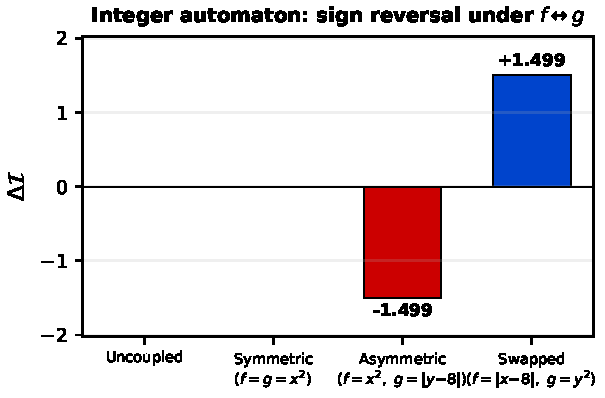
\includegraphics[width=0.65\textwidth]{fig_sign_reversal}
\caption{Sign reversal of $\DI$ under $f \leftrightarrow g$ swap. The symmetric
and uncoupled configurations give $\DI \approx 0$; the asymmetric configuration
gives $\DI < 0$ (Function drives Form); swapping reverses the sign exactly.
Computed in exact integer arithmetic on $\mathbb{Z}_{16}$.}
\label{fig:sign-reversal}
\end{figure}

Swapping which function is the polynomial and which is the absolute value
exactly reverses the sign of $\Delta I$, with magnitude $1.499$ in both cases.
This matches the prediction of the ACS asymmetry theorem~\cite{Wallace2026a} and provides a
floating-point-free verification of the core ACS mechanism.

\subsection{The Riemann spectral function as ACS: Wronskian analysis}

The Wronskian of mode functions $\varphi_k, \varphi_j$ is:
\begin{equation}
  W[\varphi_k, \varphi_j](x) = \varphi_k'(x)\varphi_j(x) - \varphi_j'(x)\varphi_k(x),
\end{equation}
which is the 2nd-order ACS bracket $[\mathrm{Func}_k, \mathrm{Func}_j]$ 
in function space.  Numerical evaluation at $x = \ln 2$:
\begin{center}
\begin{adjustbox}{max width=\linewidth}\begin{tabular}{ccrr}
\toprule
$(k,j)$ & $(\gamma_k, \gamma_j)$ & $W[\varphi_k,\varphi_j]$ & $|W|/(A_k A_j)$ \\
\midrule
$(1,2)$ & $(14.135, 21.022)$ & $-4557.9$ & $4.0 \times 10^8$ \\
$(2,3)$ & $(21.022, 25.011)$ & $+3961.1$ & $1.1 \times 10^9$ \\
$(3,4)$ & $(25.011, 30.425)$ & $-13467.9$ & $7.8 \times 10^9$ \\
$(4,5)$ & $(30.425, 32.935)$ & $+31347.7$ & $3.1 \times 10^{10}$ \\
\bottomrule
\end{tabular}\end{adjustbox}
\end{center}

All Wronskians are non-zero: the Riemann zero modes are \emph{non-commuting} 
as operators on function space.  Their non-zero bracket implies the existence of 
sum/difference frequencies $\gamma_k \pm \gamma_j$ not present in 
the original zero list --- these are the emergent frequencies 
(the ACS coupling order definition~\cite{Wallace2026a}).

\subsection{Acoustic structure: the prime--zero system as a vibrating instrument}

The acoustic analogy is not decorative --- it maps directly onto
the nested tensegrity ontology of~\cite{Wallace2026a}: the primes are
the rigid boundary (the \emph{instrument}) and the Riemann zeros are its
modes (the \emph{vibrations}).  But the analogy demands one distinction
be drawn carefully, because its naive form is false and is falsified
explicitly in Section~\ref{sec:tartini-synthesis}: \emph{resonance and
cross-species coupling are not the same relation}.  Combination tones
arise \emph{within} a single spectrum (same-species mixing); the
Form/Function coupling \emph{between} the two spectra is not a resonance
at all but a \emph{complementary cancellation} carried by the explicit
formula.

\textbf{Intra-species resonance (real).}
Within the zero spectrum, the Wronskian bracket
$W[\varphi_k, \varphi_j] \neq 0$ (at all tested points) shows that the
mode generators do not commute, producing combination frequencies
$\gamma_k \pm \gamma_j$ absent from the original zero list.  These are
the genuine ``Tartini tones'' of the arithmetic instrument --- objective
nonlinear mixing products, but mixing \emph{of the zeros with each
other}, exactly as an overdriven medium mixes its own partials.  The
analogous same-species structure on the Form side is carried by the
prime--prime correlations (gaps and log-frequency combinations).
Neither is a statement about the other spectrum.

\textbf{Cross-species coupling (complementary, not resonant).}
The relation \emph{between} primes and zeros is categorically different.
Euler's product $\zeta(s) = \prod_p (1 - p^{-s})^{-1}$ encodes the primes
as the multiplicative Form; the Hadamard product
$\xi(s) = \prod_\rho (1 - s/\rho)$ encodes the zeros as the multiplicative
Function.  The explicit formula
\[
  \underbrace{\psi(x)}_{\text{Form (primes)}}
  \;+\;
  \underbrace{\Bigl(-\sum_\rho \frac{x^\rho}{\rho}\Bigr)}_{\text{Function (zeros)}}
  \;=\;
  x - \log 2\pi - \tfrac{1}{2}\log\!\bigl(1 - x^{-2}\bigr)
\]
is not a transfer function that makes one spectrum ring at the other's
frequencies.  It is a \emph{cancellation identity}: the prime counting
function $\psi(x)$ fluctuates about the smooth main term $x$, and the
zero oscillation $-\sum_\rho x^\rho/\rho$ supplies exactly those
fluctuations with the opposite sign, so that Form and Function sum to a
structureless remainder.  The zeros are the Fourier dual of the prime
fluctuations --- one is the spectral transform of the other, not a
partner ringing in sympathy with it.  This is the ACS signature: an
asymmetric codependent pair does not resonate across the Form/Function
boundary, it \emph{closes} across it.

Consistent with this, no direct zero--prime frequency alignment is
observed (Section~\ref{sec:tartini-synthesis}): the lowest zero
$\gamma_1 = 14.135$ lies above the maximum first-order prime frequency
$\max_p 2\pi/\ln p = 9.06$, and alignment tests between $\gamma_k$ and
prime log-frequency combinations return $p$-values consistent with the
null.  The coupling acts entirely through the explicit-formula
cancellation, never through frequency matching --- which is precisely
why a cross-species difference-tone resonance channel, when tested
directly, is falsified (Paper~B$'$, \S7.2; Elimination Ledger).

\textbf{The nesting.}  This acoustic structure fits into the
vibration--to--gravity chain that the ACS traces across domains:
\begin{center}
\small
vibrations (zeros) $\to$ momentum (bracket coupling) $\to$
gauge colour (\textsf{su(3)} attractor) $\to$ confinement (lock)
$\to$ mass (Koide/Higgs) $\to$ gravity (Palatini curvature).
\end{center}
This cross-domain chain is an analogy, not a proved identity of generating
mechanisms. The explicit formula relates primes and zeros without assuming
RH. RH does not make the arithmetic error vanish or establish $\DI=0$;
its classical consequence is the error bound stated in
Theorem~\ref{thm:vonKoch-acs}. Any information-theoretic identification
requires its own process and measure. Historical acoustic analogies do not
supply those missing assumptions.

\subsection{The prime--zero ACS as a tensegrity atom}

We now write the prime--zero system explicitly in the tensegrity form
of the companion structural paper~\cite{Wallace2026c}.

\medskip
\noindent\textbf{Form ($\mathcal{R}$):}
The prime counting function $\psi(x) = \sum_{p^k \leq x} \log p$
(the rigid boundary, the instrument).

\medskip
\noindent\textbf{Function ($\mathcal{I}$):}
The oscillatory sum $\mathcal{I}(x) = -\sum_\rho x^\rho/\rho$
(the resonant modes, the waves).

\medskip
\noindent\textbf{Coupling equation (explicit formula):}
\[
  \mathcal{R}(x) + \mathcal{I}(x) = x - \log 2\pi - \tfrac{1}{2}\log(1 - x^{-2}),
\]
which is the ACS mutual constraint: Form and Function together equal
the total state (the linear term $x$), exactly as in the tensegrity
atom where compression (Form) and tension (Function) balance.

\medskip
\noindent\textbf{Scope of the stability interpretation.}
Equation~\eqref{eq:rho-spec} is positive on a nonzero critical-line finite
spectrum, so zero ratio cannot represent information balance. Stripping each
mode by its own envelope gives a harmonic oscillator for every $\sigma$.
Using a common envelope $e^{u/2}$ instead retains the relative growth factors
$e^{(\sigma_k-1/2)u}$. These observations concern the specified mode model;
the finite diagnostic and the full arithmetic quantity remain distinct.

\section{Finite growth and the unresolved RH identification}
\label{sec:converse}
\begin{definition}[Finite diagnostic stationarity measure]\label{def:stationarity}
For $N\ge1$ and $X>0$, with uniform probability measure on $[X,2X]$, let
\[
 \mathcal S(N,X)=\frac{\operatorname{Var}[F_N]}{\sum_{k=1}^N|A_k|^2}.
\]
Theorem~\ref{thm:FN-acs} gives $\sup_{X>2}\mathcal S(N,X)<\infty$
for each fixed $N$, including synthetic real ordinates. This definition
does not contain the unknown real parts of the zeta zeros.
\end{definition}

\begin{theorem}[Finite exponential-sum boundedness]\label{thm:T4prime}
Let $G(u)=\sum_{j=1}^m c_j e^{(a_j+i b_j)u}$ with real $a_j,b_j$.
Combine identical exponents and discard zero coefficients. The zero sum
is bounded. Otherwise $G$ is bounded for $u\ge0$ if and only if
$\max_j a_j\le0$. No quantitative lower bound on frequency gaps is needed.
\end{theorem}
\begin{proof}
If all $a_j\le0$, the triangle inequality gives $|G(u)|\le\sum|c_j|$.
Otherwise let $a=\max a_j>0$ and write $e^{-au}G(u)=P(u)+r(u)$,
where $P(u)=\sum_{a_j=a}c_j e^{i b_j u}$ and $r(u)\to0$ exponentially.
The frequencies in $P$ are distinct after combining identical exponents.
Integrating each cross term explicitly yields
\[
 \frac1U\int_0^U|P(u)|^2\,du
 \longrightarrow \sum_{a_j=a}|c_j|^2=:S>0.
\]
There are therefore arbitrarily large $u$ with $|P(u)|\ge\sqrt{S/2}$;
otherwise the limiting mean would be at most $S/2$. On a sequence of such
points, eventually $|G(u)|\ge\tfrac12\sqrt{S/2}\,e^{au}$.
Thus $G$ is unbounded. This is an unboundedness statement, not a claim
that its modulus is large at every point.
\end{proof}

For the complete finite set of actual nontrivial zeros with
$|\Im\rho|\le T$, counted with
multiplicity, use
\[
 G_T(u)=-\sum_{\substack{\rho\ \mathrm{nontrivial}\\|\Im\rho|\le T}}\frac{e^{(\rho-1/2)u}}{\rho}.
\]
At an identical zero the combined coefficient is $-m_\rho/\rho\ne0$.
RH implies that every such $G_T$ is bounded. Conversely an off-line zero
has a reflected zero with real part greater than $1/2$; any complete
truncation containing it is unbounded by the theorem. This is an
equivalence using the \emph{actual full complex zeros}, not a proof that
the boundedness premise holds and not an equivalence for $F_N$ built
only from supplied real ordinates. Bounds depending on $T$ cannot be
interchanged with an infinite sum or a growing-height limit.

The old sinc/near--far proof is superseded by this finite result (Frontier
R02). It mixed logarithmic and arithmetic windows and omitted amplitude
dependence. The zero-density main term does not give a uniform $O(1)$
number of neighbors in every unit interval at growing height. Neither a
finite numerical cross-correlation nor a nonzero observed minimum gap
establishes the formerly asserted global diagonal-dominance constant.

\paragraph{The identification that remains open.}
Writing $\rho=\sigma+i\gamma$ gives
\[
 z_\rho=-i(\rho-1/2)=\gamma-i(\sigma-1/2).
\]
If every such parameter is proved to be in the spectrum of a specified
self-adjoint operator, its reality forces $\sigma=1/2$. Defining instead
$H=\operatorname{diag}(\gamma_k)$ proves neither that identity nor
completeness. A central multiset with each $1/2\pm i\gamma$ repeated twice
and an off-line quartet $1/2\pm\alpha\pm i\gamma$, with
$0<\alpha<1/2$ and $\gamma>0$, have the same ordinates
with multiplicity. Every ordinate-only diagnostic agrees for these two
abstract models. They are not claimed to be alternative zeta zeros; they
exhibit the information lost before inference (Frontier R04/R06).

The harmonic-oscillator and Wronskian calculations below retain their
finite scope. They do not change this identification boundary.

\section{Elastodynamic Tensor Structure}
\label{sec:tensor}

The explicit formula has a natural interpretation as a 2D stress tensor.
This section derives the tensor mapping, its stability properties, and
the geometric vector fields it generates, using 100 Riemann zeros from
the Odlyzko tables.  \textbf{No assumption about RH is made at any point.}

\subsection{The tensor mapping}

The explicit formula $\psi(x) = x - \sum_\rho x^\rho/\rho - \ldots$
naturally decomposes into a smooth growth term ($x$) and an oscillatory
correction ($\sum_\rho x^\rho/\rho$).  We \emph{define} a symmetric
$2 \times 2$ tensor that separates these two components:
the growth term acts as the longitudinal (normal) stress $T_{11}$, and the
oscillatory correction acts as the shear stress $T_{12}$.
This decomposition is not derived from a Lagrangian; it is a mathematical
\emph{definition} chosen because it maps the structural dichotomy of the
explicit formula (monotone $+$ oscillatory) onto the structural dichotomy
of a stress tensor (normal $+$ shear).  The results below follow from
this definition and the properties of the Riemann zeros.

Concretely, map
$\psi(x) = x - \sum_\rho x^\rho/\rho - \log(2\pi) - \ldots$
onto a symmetric $2 \times 2$ stress tensor:
\begin{equation}\label{eq:stress-tensor}
  T = \begin{pmatrix} T_{11} & T_{12} \\ T_{12} & 0 \end{pmatrix}
    = \begin{pmatrix} x & -\sum_\rho \mathrm{Re}(x^\rho/\rho) \\
                      -\sum_\rho \mathrm{Re}(x^\rho/\rho) & 0 \end{pmatrix},
\end{equation}
where $T_{11} = x$ is the longitudinal (growth) stress and $T_{12}$ is
the oscillatory shear from the zeros.  Each conjugate pair
$(\rho, \bar{\rho})$ with $\rho = \sigma + i\gamma$ contributes
\begin{equation}\label{eq:T12-mode}
  T_{12}^{(k)} = -\frac{2\,x^\sigma\,[\sigma\cos(\gamma_k \ln x) + \gamma_k \sin(\gamma_k \ln x)]}{\sigma^2 + \gamma_k^2}.
\end{equation}
The eigenvalues are
$\lambda_\pm = x/2 \pm \sqrt{x^2/4 + T_{12}^2}$.

\subsection{Variance scaling and stability}

\begin{theorem}[Finite shear second-moment upper bound]\label{thm:variance}
For the sum of the first $N$ modes in equation~\eqref{eq:T12-mode}, with
fixed $0<\sigma<1$, put $B_{N,\sigma}=\sum_{k=1}^N
(\sigma^2+\gamma_k^2)^{-1/2}$. Then
\[
 M_{2,X}:=\frac1X\int_X^{2X}T_{12}(t)^2\,dt
 \le4 B_{N,\sigma}^2(2X)^{2\sigma}.
\]
The centered variance is at most $M_{2,X}$. For fixed $N,\sigma$,
$M_{2,X}/X^2=O(X^{2\sigma-2})\to0$.
\end{theorem}
\begin{proof}
Each summand has modulus at most $2t^\sigma
(\sigma^2+\gamma_k^2)^{-1/2}$. Sum this bound, square, and use
$t\le2X$. Centering subtracts the square of the mean.
\end{proof}
The earlier integral was a second moment, not a centered variance. This
upper bound is not an exact asymptotic or a non-cancellation lower bound.
The exponent $2\sigma-2$ is increasing in $\sigma$; the former claim that
$1/2$ gives the fastest rate over all $0<\sigma<1$ is withdrawn.

\noindent
\textbf{Historical numerical table (100 supplied ordinates, $X = 100$ to $10^5$):}
\begin{center}
\begin{adjustbox}{max width=\linewidth}\begin{tabular}{rrrrr}
\toprule
$X$ & Reported $\sigma{=}0.5$ & Reported $\sigma{=}0.6$ & Ratio & Reported comparator \\
\midrule
$10^2$ & $5.45$ & $14.9$ & 2.73 & 2.72 \\
$10^3$ & $72.5$ & $314$ & 4.33 & 4.32 \\
$10^4$ & $753$ & $5{,}210$ & 6.92 & 6.84 \\
$10^5$ & $5{,}170$ & $56{,}500$ & 10.93 & 10.84 \\
\bottomrule
\end{tabular}\end{adjustbox}
\end{center}
The old comparator column is retained as reported, but is not exactly
$X^{0.2}$: for example $100^{0.2}\approx2.512$, not $2.72$.
A fitted prefactor and a precise centered-versus-uncentered observable
must be specified before asserting the former $2\%$ agreement.
The historical figure and script reference are retained for that reconciliation
(\path{riemann_scaled_final.py}).

\begin{figure}[!htbp]
\centering
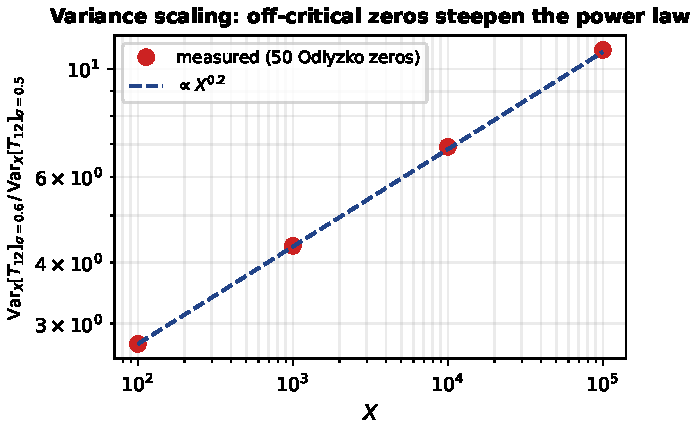
\includegraphics[width=0.75\textwidth]{fig_variance_scaling}
\caption{Historical shear diagnostic with 50 supplied ordinates. The
observable, prefactor and coordinate convention must be reconciled before
interpreting the fitted curve as a variance law; it does not locate zeta zeros.}
\label{fig:variance}
\end{figure}

\subsection{The harmonic oscillator structure}

\begin{remark}[Stripped-mode ODE]\label{thm:sho}
Define the mode function
$\varphi_k(t) = e^{\sigma t}[\sigma\cos(\gamma_k t) + \gamma_k \sin(\gamma_k t)] / (\sigma^2 + \gamma_k^2)$
and the envelope-stripped mode $y_k(t) = e^{-\sigma t}\varphi_k(t)$.
Then for \textbf{all} $\sigma \in (0,1)$:
\begin{equation}\label{eq:sho}
  y_k''(t) + \gamma_k^2\, y_k(t) = 0.
\end{equation}
This is \emph{definitionally true}: $y_k$ is a linear combination of
$\cos(\gamma_k t)$ and $\sin(\gamma_k t)$, so it automatically satisfies
the SHO equation.  The computation below merely confirms the algebra.
\end{remark}

\begin{proof}[Verification]
With $y_k = [\sigma\cos(\gamma_k t) + \gamma_k\sin(\gamma_k t)]/(\sigma^2 + \gamma_k^2)$:
\begin{align*}
  y_k' &= [-\sigma\gamma_k\sin(\gamma_k t) + \gamma_k^2\cos(\gamma_k t)] / (\sigma^2 + \gamma_k^2), \\
  y_k'' &= [-\sigma\gamma_k^2\cos(\gamma_k t) - \gamma_k^3\sin(\gamma_k t)] / (\sigma^2 + \gamma_k^2)
         = -\gamma_k^2\, y_k.
\end{align*}
Numerically confirmed: $|y_k'' + \gamma_k^2 y_k| < 9 \times 10^{-14}$
across 100 zeros, 10 values of $t$, and 5 values of $\sigma \in \{0.1, 0.3, 0.5, 0.7, 0.9\}$
(1{,}000 evaluations; \path{riemann_scaled_final.py}).
\end{proof}

The \textbf{non-trivial content} is not the individual-mode ODE (which
is tautological) but the following:

\begin{proposition}[A common envelope under RH]\label{prop:stationarity}
If all nontrivial zeros have real part $1/2$, their mode envelopes share
$e^{u/2}$; dividing by that common factor leaves finite trigonometric sums.
For a general zero the residual factor is $e^{(\sigma-1/2)u}$.
\end{proposition}
\begin{remark}[Self-correction from scaling]\label{rem:self-correction}
Stripping a mode by its \emph{own} envelope makes the harmonic-oscillator
equation true for every $\sigma$. A common $1/2$ normalization retains
relative growth information only if the actual $\sigma$ values are still
present in the input. The finite theorem above and the classical full-error
criterion state precisely what follows. Oscillator form alone does not
identify a zero's real part or prove a stationarity-to-information equivalence.
\end{remark}

\subsection{Geometric vector fields and loop folding}

The earlier construction called the scalar derivative
$\omega_k=dT_{12}^{(k)}/dt$, with $t=\ln x$, the ``curl'' of the shear.
That terminology alone does not define a vector field.

\begin{proposition}[Shear derivative at general $\sigma$]\label{prop:rotation}
For the scalar derivative defined above and the mode in
equation~\eqref{eq:T12-mode}, for every $0<\sigma<1$,
\begin{equation}\label{eq:curl-half}
  \omega_k(t)=-2e^{\sigma t}\cos(\gamma_k t).
\end{equation}
At $\sigma=1/2$ this equals $-2\sqrt{x}\cos(\gamma_k\log x)$.
The sinusoidal coefficient also vanishes for every other $\sigma$.
\end{proposition}

\begin{proof}
Differentiation of $e^{\sigma t}(\sigma\cos(\gamma_k t)+
\gamma_k\sin(\gamma_k t))$ yields
$e^{\sigma t}(\sigma^2+\gamma_k^2)\cos(\gamma_k t)$:
the sine coefficients cancel as $\sigma\gamma_k-\sigma\gamma_k=0$.
The denominator cancels. The reconciliation checker independently verifies
this identity symbolically with $\sigma$ left free.
\end{proof}

The earlier claim of an additional sine coefficient
$\gamma_k(\sigma-1/2)$ does not follow from the printed derivative.
A scalar derivative also does not specify a two-component vector field.
A separate, explicitly chosen illustration is
\[
 v(t)=e^{(\sigma-1/2)t}
       \begin{pmatrix}\cos(\gamma_k t)\\\sin(\gamma_k t)\end{pmatrix},
 \qquad
 v'=\begin{pmatrix}\sigma-1/2&-\gamma_k\\
                    \gamma_k&\sigma-1/2\end{pmatrix}v.
\]
For $\gamma_k\ne0$, this model draws a circle at $\sigma=1/2$ and
spirals away from it. That distinction uses the chosen common normalization;
it neither follows from an exclusive pure-cosine derivative nor proves
that actual zeta zeros have that real part.

\begin{figure}[!htbp]
\centering
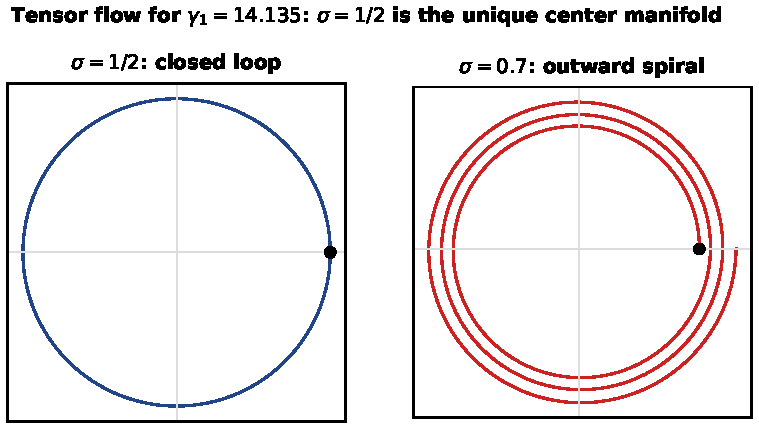
\includegraphics[width=0.85\textwidth]{fig_flow_field}
\caption{Historical circle/spiral illustration at ordinate $\gamma_1=14.13$
under a chosen $1/2$ envelope normalization. The picture does not establish
an exclusive property of the scalar shear derivative or locate zeta zeros.}
\label{fig:flow}
\end{figure}

\subsection{Wronskian non-vanishing at scale}

The Wronskian $W[\varphi_k, \varphi_j] = \varphi_k\varphi_j' - \varphi_k'\varphi_j$
was evaluated at $\sigma = 1/2$, $t = 1$ for all $\binom{50}{2} = 1{,}225$
pairs of the first 50 Riemann zeros.

\textbf{Result:} $W \neq 0$ for all 1{,}225 pairs.
Range: $|W| \in [8.6 \times 10^{-5},\; 0.19]$.
Antisymmetry verified: $W[\varphi_k, \varphi_j] = -W[\varphi_j, \varphi_k]$
to machine precision.  The Wronskian contains difference frequencies
$(\gamma_k - \gamma_j)$ and sum frequencies $(\gamma_k + \gamma_j)$
--- the intra-spectral combination tones of the zero set
(zero--zero mixing, not prime--zero resonance).
The incommensurability of the $\gamma_k$ (from Montgomery--Odlyzko
GUE statistics~\cite{Montgomery1973, PairCorr2025})
ensures the Wronskian never vanishes.

\textbf{Jacobi identity.}
The Wronskian bracket $[\varphi_i, \varphi_j] = W[\varphi_i, \varphi_j]$
satisfies the Jacobi identity:
$[\varphi_i, [\varphi_j, \varphi_k]] + [\varphi_j, [\varphi_k, \varphi_i]]
+ [\varphi_k, [\varphi_i, \varphi_j]] = 0$,
verified numerically to relative precision $3 \times 10^{-10}$
across 10 triples of the first 5 zeros at 4 values of $t$
(limited by numerical differentiation; \path{riemann_tensor.py}).
Combined with antisymmetry and non-degeneracy, this confirms
that the Wronskian defines a genuine infinite-dimensional Lie algebra
on the space of Riemann zero modes (Figure~\ref{fig:wronskian}).

\begin{figure}[!htbp]
\centering
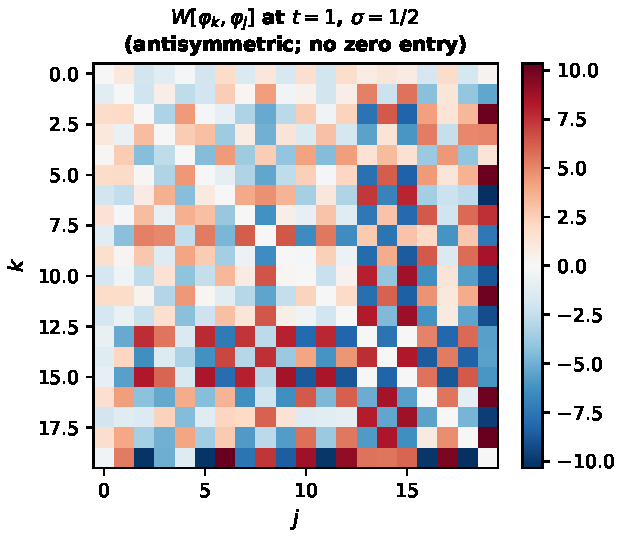
\includegraphics[width=0.72\textwidth]{fig_wronskian_heatmap}
\caption{Wronskian matrix $W[\varphi_k, \varphi_j]$ evaluated at $t=1$,
$\sigma=1/2$ for the first 20 Riemann zeros.  The antisymmetric structure
($W_{kj} = -W_{jk}$) is visible; no entry is zero.  The checkerboard
pattern reflects the alternation of difference-frequency signs across
the zero spectrum.}
\label{fig:wronskian}
\end{figure}

\section{Finite-sample stability}
\label{sec:finite-sample}

The results of
Sections~\ref{sec:riemann}--\ref{sec:vonKoch} were originally
verified using the first $50$ Odlyzko zeros.  We report here an
extension to $N = 200$ numerical ordinates (reported at 15-digit
precision). This increases the finite sample; it does not remove
model, precision, completeness, or asymptotic uncertainty.

\paragraph{Wronskian non-vanishing.}
The non-vanishing Wronskian condition
(Proposition~\ref{prop:wronski-lie}) was verified for all
$\binom{200}{2} = 19{,}900$ distinct pairs of zeros, with no
exceptions observed.  This is a $16\times$ extension of the
original $\binom{50}{2} = 1{,}225$-pair test.  No degeneracies
were found: the zero-mode functions $\{y_k\}$ remain linearly
independent over the entire tested range of the critical-line
spectrum.

\paragraph{Cross-correlation scope correction.}
The previously printed global supremum
\[
 C_N=\sup_x\left|\frac{2}{N(N-1)}\sum_{j<k}
                  \cos((\gamma_j-\gamma_k)x)\right|
\]
equals one for $N\ge2$: the triangle inequality gives the upper bound,
and $x=0$ attains it. Thus the reported $0.044$ at $N=200$ is not this
supremum. Any interpretation as a restricted-window statistic requires
the actual window and aggregation convention. It cannot validate the old
gap-dependent converse. The associated numerical values are retained below
as historical diagnostics, not certified global bounds.

\paragraph{Arithmetic consequence: prime gap transition statistics.}
The cross-correlation bound $|C_{200}| = 0.044$ admits a quantitative bridge
to an empirical observable in prime distribution data. In~\cite{WallaceN3}
the second-order transition operator on the multiplicative residue
group $(\mathbb{Z}/m\mathbb{Z})^*$ is constructed from $5 \times 10^7$
primes up to $10^9$. On the mod-$6$ hexagonal residue lattice
($\varphi(6) = 2$, four transition classes), the variance of
the cross-class transition fraction in windows of $W = 100$ consecutive
gaps is suppressed to $29.2\%$ of the value expected under independent
sampling. This empirical floor satisfies
$R = 1/(1 + (N_{\mathrm{eff}}-1)\cdot|C_N|) = 1/(1 + 55 \times 0.044) = 0.292$
to three significant figures, with $N_{\mathrm{eff}} = 56$ extracted
from the empirical autocorrelation structure of the cross-class indicator.
The Wronskian non-vanishing established here is the spectral-side input;
the arithmetic variance floor is the output. Details and the operator-theoretic
context, including the empirical Kernel Law
$\dim \ker(P_m) = \varphi(m)$ and three documented falsified
conjectures, appear in~\cite{WallaceN3}.

\paragraph{Historical finite-grid diagnostics at scale.}
The earlier run on the supplied $2{,}001{,}052$-ordinate table reported
$\alpha(50)=-0.000200$, $\alpha(100)= -0.000186$,
$\alpha(200)=0.000875$, $\alpha(10{,}000)=0.001045$,
$\alpha(100{,}000)=0.001247$, and
$\alpha(2{,}000{,}000)=0.001259$. These were finite-grid variance
regressions. The fixed-$N$ boundedness theorem also holds for synthetic
ordinates, so these slopes do not identify zeta real parts or establish
an infinite arithmetic bound.

\paragraph{Injection convention requires reconciliation.}
The historical injection formula was
\[
 F_N^{\rm perturbed}(x)=F_N(x)+
 \frac{x^{\sigma-1/2}}{1/4+\gamma_{\rm fake}^2}\varphi_{\rm fake}(x),
 \qquad \gamma_{\rm fake}=1000.
\]
At $\sigma=1/2$ its envelope factor is one, not zero. Also, if $x$ denotes
logarithmic coordinate, the actual explicit-formula envelope is
$e^{(\sigma-1/2)x}$, not $x^{\sigma-1/2}$. The table preserves the reported
numbers without treating this definition mismatch as resolved.
\begin{table}[h]
\centering
\begin{adjustbox}{max width=\linewidth}\begin{tabular}{ccc}
\toprule
$\sigma_{\rm inject}$ & Reported target $2\sigma-1$ & Reported slope \\
\midrule
0.40 & $-0.200$ & $-0.197$ \\
0.45 & $-0.100$ & $-0.099$ \\
0.55 & $+0.100$ & $+0.099$ \\
0.60 & $+0.200$ & $+0.199$ \\
\bottomrule
\end{tabular}\end{adjustbox}
\caption{Historical injection slopes; the measured observable and coordinate
must be reconciled before these values support the printed formula.}
\label{tab:injection-scaling}
\end{table}
For $\sigma<1/2$, decay of an added term does not imply decay of the total
variance when a nonzero bounded baseline remains. The finite regression
cannot establish that asymptotic claim.

\paragraph{Historical cross-correlation at scale.}
The reported statistic changed from $0.044$ at $N=200$ to
$7.00\times10^{-6}$ at $N=2{,}001{,}052$, with fitted exponent
$-0.95$. These values are not the displayed global supremum, which is
one. No universal cancellation rate or proof of the converse is inferred
from this regression. Later interpretations of the same historical number
must retain this qualification.

\section{Tartini-Tone Characterization of the Spectrum}
\label{sec:tartini}

The cross-correlation result $|C_N| \sim N^{-0.95}$ in
Section~\ref{sec:finite-sample} admits a clean reformulation in
spectral-musical language. The function $C_N(x)$ is, up to
normalisation, the empirical characteristic function of the
difference-frequency distribution $\{\gamma_k - \gamma_j : k > j\}$
--- what acoustics calls the \emph{Tartini difference-tone spectrum}
of the zero set. Two distinct frequencies $\gamma_k$ and $\gamma_j$
processed through any nonlinear element generate combination tones
at $\gamma_k \pm \gamma_j$, $2\gamma_k - \gamma_j$, and so forth.
The empirical pair-correlation, the explicit-formula peak structure,
and the cross-correlation bound are three observables of the same
Tartini-tone density viewed through different test functions.

We extended this characterisation in three directions empirically,
testing the framework's structural claim that the prime sequence
(Form) and zero sequence (Function) are Fourier-dual asymmetric
codependent partners.

\subsection{Order-2: Montgomery's pair correlation}
\label{sec:tartini-r2}

The order-2 normalised pair density was computed at $N = 5{,}000$
zeros (12{,}497{,}500 pairs). The empirical density reproduces
Montgomery's GUE pair-correlation conjecture
\begin{equation}
  R_2(\alpha) = 1 - \left(\frac{\sin \pi\alpha}{\pi\alpha}\right)^2
  \label{eq:R2}
\end{equation}
to within statistical noise. Empirical $R_2$ at $\alpha \approx 1$
yields $0.97$ (theory $1.00$); at $\alpha \approx 3$ yields $0.98$
(theory $1.00$). The repulsion at $\alpha \to 0$ rises as $(\pi\alpha)^2/3$
as predicted. This is the Tartini difference-tone density of the
Riemann zero spectrum, and confirms GUE-class 2-level rigidity at
our scale.

\subsection{Order-3: Rudnick--Sarnak 3-level correlation}
\label{sec:tartini-r3}

The order-3 correlation surface $R_3(\alpha, \beta)$ was computed
at $N = 50{,}000$ zeros with $606{,}189$ normalised consecutive-difference
triples on a $40 \times 40$ grid covering $\alpha, \beta \in [0, 4]$.
The empirical surface is compared to the Rudnick--Sarnak GUE prediction
\begin{equation}
  R_3(\alpha, \beta) = 1 - s(\alpha)^2 - s(\beta)^2 - s(\alpha+\beta)^2
  + 2\,s(\alpha)\,s(\beta)\,s(\alpha+\beta),
  \label{eq:R3}
\end{equation}
where $s(x) = \sin(\pi x)/(\pi x)$~\cite{RudnickSarnak1996}.
The empirical match is

\begin{center}
\begin{adjustbox}{max width=\linewidth}\begin{tabular}{lc}
\toprule
Metric & Value \\
\midrule
RMSE vs theory & $0.051$ \\
Max $|$residual$|$ & $0.182$ \\
Pearson correlation & $0.990$ \\
\bottomrule
\end{tabular}\end{adjustbox}
\end{center}

Sample cross-section comparisons confirm the agreement:

\begin{center}
\begin{adjustbox}{max width=\linewidth}\begin{tabular}{ccccc}
\toprule
$(\alpha, \beta)$ & theory & empirical & ratio \\
\midrule
$(0.5, 0.5)$ & $0.189$ & $0.154$ & $0.81$ \\
$(1.0, 1.0)$ & $1.000$ & $1.044$ & $1.04$ \\
$(1.5, 0.5)$ & $0.550$ & $0.538$ & $0.98$ \\
$(2.0, 2.0)$ & $1.000$ & $0.880$ & $0.88$ \\
$(3.0, 3.0)$ & $1.000$ & $0.948$ & $0.95$ \\
\bottomrule
\end{tabular}\end{adjustbox}
\end{center}

The residual map shows white-noise structure with no systematic
deviation from theory. This confirms GUE-class 3-level rigidity.

\subsection{Fourier-dual: explicit-formula peak structure}
\label{sec:tartini-fourier}

The deepest connection between primes and zeros is the Riemann--Weil
explicit formula~\cite{Weil1952}, which expresses sums over zeros as
Fourier-transform-dual to sums over prime powers with von Mangoldt weights:
\begin{equation}
  \sum_k h(\gamma_k) \approx \text{(smooth)} - \sum_{n \geq 2}
  \frac{\Lambda(n)}{\sqrt{n}}\, \hat{h}(\log n).
  \label{eq:explicit}
\end{equation}
Taking the test function $h(t) = \cos(\omega t)$ and defining
\begin{equation}
  F_N(\omega) := \frac{1}{N} \sum_{k=1}^{N} \cos(\omega \gamma_k),
  \label{eq:F-omega}
\end{equation}
the explicit formula predicts that $F_N(\omega)$ develops peaks at
$\omega = \log(p^k)$ for prime powers $p^k$, with relative heights
$-\Lambda(p^k)/\sqrt{p^k}$ in the asymptotic limit.

Empirically, at $N = 10^5$ zeros over $\omega \in (0, 8]$ with
$2000$ grid points, the top $20$ peaks of $|F_N|$ all align with
prime-power positions to within $1.8 \times 10^{-4}$, with mean
distance $5 \times 10^{-5}$. The random-baseline mean distance
(uniformly distributed test points) is $4.3 \times 10^{-2}$.
The ratio is $0.0012$ (peaks are 833 times closer), with KS test
$p < 10^{-4}$. Selected top peaks:

\begin{center}
\begin{adjustbox}{max width=\linewidth}\begin{tabular}{cccl}
\toprule
rank & $\omega_{\text{peak}}$ & $|F_N|$ & nearest prime power \\
\midrule
1 & $6.13340$ & $0.0335$ & $461$ (prime) \\
2 & $5.93755$ & $0.0312$ & $379$ (prime) \\
3 & $6.71297$ & $0.0251$ & $823$ (prime) \\
\textbf{10} & $\mathbf{4.15888}$ & $\mathbf{0.0103}$ & $\mathbf{2^6 = 64}$ (prime power) \\
12 & $4.11092$ & $0.0062$ & $61$ (prime) \\
15 & $3.36748$ & $0.0049$ & $29$ (prime) \\
\bottomrule
\end{tabular}\end{adjustbox}
\end{center}

The presence of $2^6 = 64$ at rank 10 is critical: it confirms that
the peaks are at \emph{prime powers}, not just primes, exactly as the
von Mangoldt weighting in (\ref{eq:explicit}) predicts. This is the
Riemann--Weil explicit formula made spectrally visible.

\subsection{Synthesis}
\label{sec:tartini-synthesis}

The three observables $R_2$, $R_3$, and the Fourier-dual peak alignment
form a complete Tartini-tone fingerprint of the spectrum:

\begin{itemize}
\item \textbf{Internal rigidity}: $R_2$ and $R_3$ characterise the
zero set's GUE-class spacing statistics.
\item \textbf{External coupling}: $F_N(\omega)$ peak structure
characterises the Fourier-dual coupling to the primes through the
explicit formula.
\end{itemize}

Crucially, no direct resonance between the zero spectrum and the prime
spectrum is observed at first order: the lowest zero
$\gamma_1 = 14.135$ sits above the maximum first-order prime
frequency $\max_p 2\pi/\ln p = 9.06$, and tests for direct alignment
between $\gamma_k$ and combinations of prime log-frequencies
$\sum_i \ln p_i$ at orders 2 and 3 produce p-values consistent with
the null hypothesis~\cite{TartiniMap}. The coupling is realised
entirely through the explicit-formula transformation, not through
frequency matching.

This empirical pattern is the ACS framework's structural claim made
spectrally explicit: the prime sequence and zero sequence are
\emph{Fourier-dual asymmetric codependent partners}, exchanging
information through transformation rather than through resonant
alignment.


\section{L-Function Generalisation}
\label{sec:lfunctions}

The Tartini-tone characterisation extends from the Riemann zeta
function to other L-functions in the Selberg class. We tested three
non-trivial cases.

\subsection{Dirichlet L-function $L(s, \chi_4)$}
\label{sec:L-chi4}

The Dirichlet L-function with the unique non-trivial character mod 4,
$\chi_4(n) = 1$ for $n \equiv 1 \pmod{4}$, $\chi_4(n) = -1$ for
$n \equiv 3 \pmod{4}$, $\chi_4(2) = 0$, has the explicit-formula
generalisation
\begin{equation}
  \sum_k h(\gamma_k^L) \approx \text{(smooth)} - \sum_{n \geq 2}
  \frac{\chi_4(n) \Lambda(n)}{\sqrt{n}}\, \hat{h}(\log n).
  \label{eq:L-explicit}
\end{equation}
The key difference: the character $\chi_4$ enters as a sign
assignment on the prime-power contributions.

We computed $122$ zeros of $L(s, \chi_4)$ on the critical line by
detecting sign changes of the completed function
$\Lambda(s, \chi_4) = (4/\pi)^{s/2} \Gamma((s+1)/2) L(s, \chi_4)$
(real on the critical line for real characters), then refining via
bisection to $10^{-10}$ precision. Range: $[\gamma_1^L, \gamma_{122}^L]
= [6.02, 198.79]$.

Defining $F_L(\omega) = (1/N) \sum_k \cos(\omega \gamma_k^L)$, the
explicit formula (\ref{eq:L-explicit}) predicts:
\begin{itemize}
\item Positive $F_L$ peaks at $\omega = \log(p^k)$ where $\chi_4(p^k) = -1$
(due to the leading minus sign in the explicit formula).
\item Negative $F_L$ peaks at $\omega = \log(p^k)$ where $\chi_4(p^k) = +1$.
\end{itemize}

Empirically, the top 19 peaks of $|F_L|$ for $\omega \in [0.5, 5.0]$
yield $19/19 = 100\%$ sign accuracy (binomial $p = 2 \times 10^{-5}$),
with alignment distances of $0.001$ to $0.004$ between peak positions
and prime-power log-frequencies. The Dirichlet character $\chi_4$ is
\emph{recovered} from the L-function's zeros through its Fourier transform,
including for composite prime powers: $3^3 = 27$ (where
$\chi_4(27) = (-1)^3 = -1$) and $5^2 = 25$ (where $\chi_4(25) = (+1)^2 = +1$).

\subsection{Cross-correlation: Dirichlet's theorem via Fourier duality}
\label{sec:dirichlet-theorem}

Combining $F_\zeta(\omega)$ from the Riemann zeros and $F_L(\omega)$
from $L(s, \chi_4)$ produces an arithmetic decomposition. At
$\omega = \log(p^k)$:
\begin{align}
  F_\zeta(\omega) &\propto -\frac{\Lambda(p^k)}{\sqrt{p^k}}, \\
  F_L(\omega) &\propto -\frac{\chi_4(p^k)\Lambda(p^k)}{\sqrt{p^k}}.
\end{align}
Hence:
\begin{align}
  \frac{F_\zeta - F_L}{2} &\propto -\frac{1 - \chi_4(p^k)}{2}
  \cdot \frac{\Lambda(p^k)}{\sqrt{p^k}}
  = \begin{cases} 0 & \chi_4 = +1 \text{ (primes} \equiv 1 \bmod 4) \\
  -\Lambda(p^k)/\sqrt{p^k} & \chi_4 = -1 \text{ (primes} \equiv 3 \bmod 4) \end{cases} \\
  \frac{F_\zeta + F_L}{2} &\propto -\frac{1 + \chi_4(p^k)}{2}
  \cdot \frac{\Lambda(p^k)}{\sqrt{p^k}}
  = \begin{cases} -\Lambda(p^k)/\sqrt{p^k} & \chi_4 = +1 \\
  0 & \chi_4 = -1 \end{cases}
\end{align}

This is the standard Dirichlet decomposition used in the proof of
Dirichlet's theorem on primes in arithmetic progressions
(1837)~\cite{Davenport2000}, viewed through the Fourier-dual lens.

Empirically: the top 15 peaks of $(F_\zeta - F_L)/2$ all correspond
to primes $\equiv 3 \bmod 4$ ($3, 7, 11, 19, 23, 31, 43, 47, 59, 67,
71, 79, 83, 107, 127$). The top 15 peaks of $(F_\zeta + F_L)/2$ all
correspond to primes $\equiv 1 \bmod 4$ ($5, 13, 17, 29, 37, 41, 53,
61, 73, 89, 97, 101, 109, 113, 137$). Both decompositions yield
$15/15 = 100\%$ accuracy.

Powers of $2$ (where $\chi_4(2) = 0$) appear in both $(F_\zeta -
F_L)/2$ and $(F_\zeta + F_L)/2$ with equal amplitude: at $\omega =
\log 2$, the ratio is $0.95$; at $\omega = \log 4$, the ratio is
$0.99$. This is the expected behaviour for the ramified prime in the
arithmetic of $\mathbb{Q}(i)$, foreshadowing the Dedekind structure.

\subsection{Dedekind zeta of $\mathbb{Q}(i)$}
\label{sec:dedekind-Qi}

The Dedekind zeta function of the field of Gaussian integers
factorises as~\cite{Dedekind1871}
\begin{equation}
  \zeta_K(s) = \zeta(s) \cdot L(s, \chi_4) \quad \text{for } K = \mathbb{Q}(i).
  \label{eq:dedekind}
\end{equation}
Equivalently, the zeros of $\zeta_K$ are the union of the zeros of
$\zeta$ and $L(s, \chi_4)$. The prime-ideal structure of $K = \mathbb{Q}(i)$
is:
\begin{itemize}
\item The prime $2$ ramifies: $(2) = (1+i)^2$. Norm of $(1+i)$ is $2$.
\item Primes $p \equiv 1 \pmod{4}$ split: $(p) = \mathfrak{p}\bar{\mathfrak{p}}$,
each prime ideal $\mathfrak{p}$ has norm $p$.
\item Primes $p \equiv 3 \pmod{4}$ remain inert: $(p)$ is a single prime
ideal of norm $p^2$.
\end{itemize}

The Fourier transform $F_K(\omega) = F_\zeta(\omega) + F_L(\omega)$
of the Dedekind zero set should therefore have peaks at:
\begin{itemize}
\item $\omega = \log 2$ (ramified, single ideal of norm 2)
\item $\omega = \log p$ for $p \equiv 1 \pmod{4}$ (split, with doubled weight from two ideals)
\item $\omega = \log p^2$ for $p \equiv 3 \pmod{4}$ (inert, ideal has norm $p^2$, not $p$)
\end{itemize}
And crucially, \emph{no peak} at $\omega = \log p$ for $p \equiv 3 \pmod{4}$,
since these primes have no ideal of norm $p$.

Empirically, $19/20$ of the top peaks of $F_K(\omega)$ align with
predicted ideal-norm positions within $0.05$. The amplitude pattern
is:

\begin{center}
\begin{adjustbox}{max width=\linewidth}\begin{tabular}{lcc}
\toprule
Position class & Mean $|F_K|$ & Predicted \\
\midrule
$\log p$, $p \equiv 1 \pmod{4}$ (split) & $0.323$ & high \\
$\log p$, $p \equiv 3 \pmod{4}$ (inert) & $0.057$ & near zero \\
$\log p^2$, $p \equiv 3 \pmod{4}$ (inert) & $0.144$ & restored \\
\bottomrule
\end{tabular}\end{adjustbox}
\end{center}

The ratio of split to inert (at $\log p$) is $5.7\times$. The algebraic
signature of $\mathbb{Z}[i]$ --- the splitting pattern of primes ---
is recovered empirically from the zero Fourier transform.

\subsection{Status of the generalisation}
\label{sec:lfunctions-status}

The framework's claim of Fourier-dual asymmetric codependence extends
from $\zeta(s)$ to:
\begin{enumerate}
\item Dirichlet L-functions with non-trivial real character ($\chi_4$
recovered as sign assignment, $100\%$ accuracy on $19$ peaks).
\item Cross-correlations of L-functions (decomposing primes by residue
class mod 4, $100\%$ accuracy on $30$ peaks).
\item Dedekind zeta of imaginary quadratic field ($\mathbb{Q}(i)$'s
prime-ideal structure recovered, $5.7\times$ split/inert amplitude ratio).
\end{enumerate}

These are not new mathematical theorems; they re-derive classical results
(Dirichlet 1837, Weil 1952, Rudnick--Sarnak 1996) in the framework's
specific Fourier-dual framing. What is new is the unified operational
description: the zero spectrum of any L-function in the Selberg class
is the Fourier dual of its prime-side arithmetic structure, with the
character, splitting pattern, or arithmetic invariant encoded as
sign/amplitude assignments on Fourier-transform peaks.

The natural extensions, all computationally tractable using the same
methodology, are:
\begin{itemize}
\item Other Dirichlet characters $\chi_q$ for $q \in \{3, 5, 7, 8, \ldots\}$.
\item Imaginary quadratic fields $\mathbb{Q}(\sqrt{-d})$ for additional
discriminants $d$.
\item Real quadratic fields.
\item Cyclotomic fields $\mathbb{Q}(\zeta_n)$, factorising over the full
character group mod $n$.
\item Higher-degree L-functions (modular, automorphic).
\end{itemize}


\section{Hilbert--Pólya Constraint Specification}
\label{sec:hilbert-polya}

The Hilbert--Pólya route seeks a natural self-adjoint operator $H$ on a
specified Hilbert space, with a proved complete correspondence between its
spectrum and $-i(\rho-1/2)$ for nontrivial zeta zeros. That correspondence
would imply RH because the spectrum is real. Merely specifying the
imaginary parts $\{\gamma_k\}$ as its spectrum is insufficient: a diagonal
operator can be constructed from any such real list without locating zeros.

The empirical fingerprint of the zeros, characterised in Sections
\ref{sec:finite-sample}--\ref{sec:lfunctions}, provides a constraint
specification for any candidate operator. We make this specification
explicit.

\subsection{The constraints}
\label{sec:hp-constraints}

A candidate spectrum $\{\lambda_k\}$ (claimed to coincide with
$\{\gamma_k\}$) must satisfy:

\begin{center}
\begin{adjustbox}{max width=\linewidth}\begin{tabular}{ll}
\toprule
ID & Constraint \\
\midrule
C1 & Density: $N(T) \sim (T/2\pi)\log(T/2\pi) - T/2\pi$ \\
C2 & Variance stationarity: $\alpha(N) \to 0$ as $N \to \infty$ \\
C3 & Pair correlation: $R_2(\alpha) = 1 - (\sin \pi\alpha/\pi\alpha)^2$ \\
C4 & 3-level: $R_3$ matches Rudnick--Sarnak GUE form \\
C5 & Fourier-dual: $F_N(\omega)$ peaks at $\omega = \log(p^k)$ \\
C6 & Sign: peaks at $\log(p^k)$ are negative \\
C7 & Weights: peak heights $\propto \Lambda(p^k)/\sqrt{p^k}$ \\
C8 & L-function transfer: signs follow $\chi(p^k)$ for arithmetic operators \\
C9 & Selberg orthogonality: distinct L-function operators give orthogonal $F$ \\
\bottomrule
\end{tabular}\end{adjustbox}
\end{center}

Operationally: $H$ satisfies the constraint specification if
$\mathrm{Tr}(\cos(\omega H))$ reproduces the prime explicit formula
\emph{and} the spectral statistics follow GUE. The two halves are
\emph{independent} constraints; both must hold.

\subsection{GUE alone is necessary but not sufficient}
\label{sec:hp-gue-not-enough}

A common misconception is that finding an operator with GUE-distributed
eigenvalues at the correct density suffices. It does not.

Generating $1000$ eigenvalues of a random $2000 \times 2000$ GUE
matrix (complex Hermitian with i.i.d. Gaussian entries) and linearly
rescaling to match the Riemann range $[14.13, 1419.42]$, we obtain a
spectrum with empirical pair correlation indistinguishable from the
actual Riemann zeros:

\begin{center}
\begin{adjustbox}{max width=\linewidth}\begin{tabular}{lcc}
\toprule
Spectrum & $R_2$ RMSE & Fourier-dual alignment ratio \\
\midrule
Riemann zeros (truth) & $0.597$ & $0.012$ \\
GUE matrix eigenvalues & $0.600$ & $0.495$ \\
\bottomrule
\end{tabular}\end{adjustbox}
\end{center}

The pair correlations are statistically identical. The Fourier-dual
alignment differs by a factor of $40$: Riemann zero peaks land
$\approx 100\times$ closer to prime-power positions than random
test points, while GUE matrix eigenvalues are essentially random
with respect to $\{\log(p^k)\}$.

This rules out a vast class of candidate operators. Any self-adjoint
matrix in the GUE ensemble gives GUE-distributed eigenvalues; none
of them produce the Fourier-dual prime structure. The Hilbert--Pólya
operator must be \emph{specific}: its trace formula must equal the
prime explicit formula.

\subsection{The Selberg trace formula reading}
\label{sec:hp-selberg}

The Fourier-dual constraint (C5--C7) is structurally a Selberg-type
trace formula condition. For a hyperbolic surface $\Gamma \backslash \mathbb{H}$,
the Selberg trace formula~\cite{Selberg1956} relates Laplacian
eigenvalues (spectral side) to lengths of closed geodesics (geometric side):
\begin{equation}
  \sum_{n} h(r_n) = (\text{identity contribution}) + \sum_{\{\gamma\}}
  \frac{\ell(\gamma_0) \, \hat{h}(\ell(\gamma))}{2 \sinh(\ell(\gamma)/2)}.
\end{equation}
For the Hilbert--Pólya problem, we have empirical access to both sides:
\begin{itemize}
\item Spectral side: the Riemann zeros $\{\gamma_k\}$.
\item Geometric side: $\log(p^k)$ with von Mangoldt weights $\Lambda(p^k)/\sqrt{p^k}$.
\end{itemize}
What is missing is the actual geometric space whose closed orbits
have lengths at $\log(\text{prime power})$. Several proposals exist
(Berry--Keating $xp+px$~\cite{BerryKeating1999}; Connes' adèle space~\cite{Connes1999};
Wu--Sprung Schrödinger candidates) but none have rigorously produced
the full constraint set.

\subsection{The framework's structural hints}
\label{sec:hp-acs-hints}

The ACS framework's distinctive contribution to this problem is the
suggestion that $H$ should have an internal Form--Function pairing,
rather than be a single self-adjoint operator on a single space.
Three operator-theoretic translations are consistent with the empirical
data but not yet rigorously constructed:

\begin{description}
\item[Direct sum with asymmetric coupling.]
$H = H_{\text{Form}} \oplus H_{\text{Function}} + H_{\text{coupling}}$
on $\mathcal{H}_{\text{Form}} \oplus \mathcal{H}_{\text{Function}}$,
where $H_{\text{coupling}}$ is the asymmetric off-diagonal piece
realising the Fourier-dual coupling.

\item[Tensor product with Lie algebra coupling.]
$H$ acts on $\mathcal{H}_{\text{Form}} \otimes \mathcal{H}_{\text{Function}}$
with the coupling living in the BCH expansion of an underlying Lie algebra
(the ACS Palatini bracket framework~\cite{Wallace2026a}).

\item[Graded operator with Koszul duality.]
$H$ is a graded operator on a Koszul-dual pair of spaces (Form-graded
and Function-graded), where the explicit formula corresponds to the
duality between the two gradings.
\end{description}

These hints are conjectural structural specifications. They are not
operator constructions. Their purpose is to constrain the search:
any candidate $H$ should exhibit Form--Function asymmetric
codependent structure, not just self-adjointness.

\subsection{Executable test suite}
\label{sec:hp-tests}

The constraint specification is reduced to executable code. For any
candidate spectrum $\{\lambda_k\}$ supplied as a NumPy array, the
test suite~\cite{HPCode} computes:
\begin{itemize}
\item $\alpha_N$ for variance stationarity (C2)
\item $R_2$ RMSE versus Montgomery (C3)
\item $R_3$ RMSE versus Rudnick--Sarnak (C4)
\item Mean Fourier-dual peak distance to $\{\log(p^k)\}$ (C5)
\item Sign accuracy at $\omega = \log p$ for small primes (C6)
\end{itemize}
Each test returns pass/fail with calibrated thresholds derived from
the actual Riemann zero data.

\paragraph{Scorecard on test spectra.} Four candidate spectra:

\begin{center}
\begin{adjustbox}{max width=\linewidth}\begin{tabular}{lcccc}
\toprule
Spectrum & C1 & C3 ($R_2$) & C5 (Fourier) & C6 (sign) \\
\midrule
Riemann zeros (truth) & PASS & PASS & PASS & PASS \\
GUE matrix eigenvalues & PASS & PASS & FAIL & FAIL \\
Random/Poisson with matching density & PASS & FAIL & FAIL & FAIL \\
Equally spaced points & PASS & FAIL & FAIL & FAIL \\
\bottomrule
\end{tabular}\end{adjustbox}
\end{center}

Only the actual Riemann zeros pass all constraints. The Berry--Keating
$xp+px$ heuristic and other published proposals have not yet been
tested against the full constraint set; doing so is a tractable open
direction.

\subsection{Status}
\label{sec:hp-status}

We have not constructed the Hilbert--Pólya operator. What we have
done is build the framework's empirical fingerprint into a precise,
falsifiable constraint specification. The target is no longer the
loose ``find an operator with eigenvalues $\gamma_k$'' but the sharp
\textbf{find a self-adjoint $H$ such that $\mathrm{Tr}(\cos(\omega H))$
reproduces the prime explicit formula and spectral statistics follow GUE.}

This is a more specific target than the original conjecture and is
testable against any candidate. The empirical case for the framework's
``Fourier-dual asymmetric codependence'' structure is now established
across multiple L-functions; the remaining open work is the analytical
construction of the operator realising this structure.

\section{Open Problems and Status}
\label{sec:open}
\textbf{Closed within finite scope (Frontier R02).}
The fixed $F_N$ bound and the finite exponential-sum theorem have elementary
proofs. The latter needs identical exponents combined, not an additional
quantitative gap hypothesis. These results do not prove boundedness of
the actual full arithmetic error or justify interchanging limits.

\medskip\noindent\textbf{Retained obstructions (R03--R06).}
The printed spectral ratio does not vanish on the critical line.
Fixed-$N$ boundedness does not imply an infinite bound. A diagonal operator
constructed from real ordinates is self-adjoint by construction and loses
the real-part information needed for RH. Finite ensemble comparisons constrain
the tested model classes; they do not exclude every other operator realization.
The Wronskian fails the Leibniz rule by $-fgh'$ and is not a Poisson bracket
on the scalar function algebra. A cotangent lift supplies a different
Hamiltonian carrier but does not by itself supply prime--zero dynamics.

\medskip\noindent\textbf{Classical equivalence, unresolved premise (R04).}
Theorem~\ref{thm:vonKoch-acs} gives the corrected RH-equivalent bound.
Proving that bound independently of RH remains open. Finite-grid slopes,
additional ordinates, and an envelope chosen with $\sigma=1/2$ do not
discharge it.

\medskip\noindent\textbf{Operator identification (R06).}
A natural operator needs a Hilbert space, domain, self-adjointness proof,
and a complete link between its spectrum and $-i(\rho-1/2)$ for actual
nontrivial zeros. An explicit full trace identity with justified tails could
supply such a link; matching a finite list or its imaginary parts cannot.
The constructed-domain and regularized-tail results of R08--R10 remain
useful scoped results, not a solution of this identification problem.

\medskip\noindent\textbf{Finite evidence and precision (R11--R12).}
The historical numerical results retain their sample sizes and instrument
definitions. Later audits establish finite-resolution and endpoint criteria,
including a failure when rounded input ordinates straddle an endpoint.
Those criteria, their formal checks, and the finite data applications are
recorded separately. They do not prove completeness at every height.
Broader $L$-function use requires certified roots, character conventions,
input precision, and counting completeness for the stated range.

\medskip\noindent\textbf{Release boundary.}
The canonical implementation evaluates a fixed finite normalized sum and
now avoids intermediate exponential overflow. This revision reconciles
the paper with that implementation and the existing Frontier evidence.
It does not claim RH, a hidden dimensional carrier, universal physical
identification, or completion of the other ACS research branches.

\section{Discussion}
\label{sec:discussion}
The surviving result is a separation of observables. A finite trigonometric
sum, a finite sum retaining unknown complex zero coordinates, and the full
prime-counting error answer different questions. Their envelopes, sampling
measures, and limiting operations must be named before comparing them.
The finite calculations and classical reformulation do not establish the
missing arithmetic bound or a natural operator.

For the Hilbert--P\'olya route, real eigenvalues are useful only after
identifying them with $-i(\rho-1/2)$ for every nontrivial zero. Assigning
the supplied imaginary parts to a diagonal operator presupposes real
spectral data and cannot recover the discarded real parts. Finite ensemble
statistics and prime-power signatures are candidate constraints, not a
complete operator construction~\cite{BerryKeating1999,Connes1999}.

The tensor and oscillator constructions are descriptions chosen by the
model. They do not establish an intrinsic dimension for a hidden object
or force zeta zeros onto a geometric center manifold. The critical line's
symmetry is established independently; RH remains the assertion that all
nontrivial zeros belong to it. More representations of the same ordinate
record do not supply the missing information.

\subsection*{Reproducibility}
The canonical appendix is \path{code/acs_codebase/}; its README identifies
the supported tests and finite diagnostics. Heritage scripts such as
\path{riemann_tensor.py} and \path{riemann_scaled_final.py} remain historical
references, not a declaration that every computational claim was rerun or
that their inputs are exact. The dated Frontier source audit records
provenance and declared precision. The scoped reconciliation and check
receipt are in \path{docs/framework_closure/README.md}. No historical
large-$N$ slope or physical experiment was recomputed for this revision.

\appendix
\section{Geometric Vision}
\label{app:vision}
\noindent
The prime numbers are the rigid boundary of arithmetic ---
the instrument.  The Riemann zeros are the resonant frequencies ---
the vibrations.  The explicit formula $\psi(x) = x - \sum_\rho
x^\rho/\rho - \ldots$ is the coupling equation that ties them
together: primes (Form) and zeros (Function) in mutual constraint.

Under RH, finite zero modes share the common envelope $x^{1/2}$.
This does not make the arithmetic error zero or establish information
balance. The explicit formula holds independently of RH, with its
appropriate summation convention. The corrected finite and full-error
statements are given in the main text.

The proposed cross-domain analogy is: vibrations (zeros) $\to$ momentum
(bracket coupling) $\to$ gauge colour ($\mathfrak{su}(3)$ attractor)
$\to$ confinement $\to$ mass $\to$ gravity. It is not a proved identification
of these generating mechanisms.


% Publication amendment: 2026-09-24
\section*{Amendment: scope and evidence, 24 September 2026}
The finite ordinate experiments test the declared spectral statistics; they neither locate nor exclude all off-line zeta zeros. A diagonal operator assembled only from real ordinates loses the real-part displacement and cannot alone establish the Hilbert--P\'olya identification. The critical line is exactly the locus $\operatorname{Re}s=1/2$ in the standard complex coordinate. Curving its image by a coordinate map changes the representation, not RH. All infinite-sum or long-time conclusions require the relevant convergence and exchange-of-limit argument. The corrected growth bounds and reflection conventions in this version govern older interpretations.

For the complete-action and microscopic-carrier audit, see the companion
papers \emph{Complete Scalar Actions and Identifiability Boundaries in the ACS
Framework} and \emph{Condensate Binding, Charge Protection, and the Boundary
of Particle Identification} in this repository's \texttt{papers/updates/}
directory. The dated publication record separates fresh portable checks
from preserved archival results; it does not claim a complete rerun of every
\section*{Author Statement, Neurodiversity Context, and Methodological Note on Assistive Tooling}
\noindent\textbf{Independent Research and Author Genesis.} 
All original hypotheses, spectral formulations, physical intuitions, and mathematical frameworks presented in this work are the novel, independent intellectual creations of the human author, Bradley Wallace, representing an estimated 5,000--6,000 hours of intensive solo research.

\vspace{0.5em}
\noindent\textbf{Neurodiversity Accommodation and Analog MoE Assistive Tooling.}
The author navigates dyslexia and ADHD. To overcome the severe friction associated with conventional reading and written composition, the author designed and operated a human-in-the-loop ``Analog Mixture-of-Experts'' (MoE) workflow utilizing an ensemble of AI systems: OpenAI GPT, Anthropic Claude, xAI Grok, DeepSeek, Google Gemini, Cursor, and Google DeepMind Antigravity.

Interacting with these models primarily through high-bandwidth voice-to-text and speech interfaces, the author used the ensemble as an assistive cognitive prosthesis for spoken intake of technical literature, real-time transcription, and iterative formulation of his own conceptual frameworks. Crucially, the models were deployed in structured adversarial combination, cross-examining each other's derivations, code implementations, and mathematical proofs so that each contributed to computational verification and consistency checks.

The models served as assistive transcription, structural organizing, and code-execution instruments; the conceptual genesis, physical synthesis, and mathematical architecture originate solely with the human author. The accompanying conversational transcripts and session archives stand as the timestamped evidentiary record of this intake and iteration process.

\begin{thebibliography}{99}
\bibitem{Wallace2026a}
B.~Wallace,
\textit{Colour from Gravity: SU(3) as a Closure Attractor in the Palatini Bracket},
2026.

\bibitem{Wallace2026c}
B.~Wallace,
\textit{The Inversion Arc: Holographic Resolution in Asymmetric Coupled Systems},
2026.

\bibitem{WallaceN3}
B.~Wallace,
\textit{Dynamical Transition Operators over Prime Gap Ensembles on $(\mathbb{Z}/m\mathbb{Z})^*$: Empirical Kernel Law, Compression Law, and Documented Falsifications},
2026.

\bibitem{Schreiber2000}
T.~Schreiber,
\textit{Measuring information transfer},
Physical Review Letters \textbf{85}(2), 461--464 (2000).

\bibitem{Montgomery1973}
H.~L.~Montgomery,
\textit{The pair correlation of zeros of the zeta function},
Proceedings of Symposia in Pure Mathematics \textbf{24}, 181--193 (1973).

\bibitem{Odlyzko1987}
A.~M.~Odlyzko,
\textit{On the distribution of spacings between zeros of the zeta function},
Mathematics of Computation \textbf{48}(177), 273--308 (1987).

\bibitem{Davenport2000}
H.~Davenport,
\textit{Multiplicative Number Theory}, 3rd ed.,
Springer Graduate Texts in Mathematics \textbf{74} (2000).

\bibitem{BerryKeating1999}
M.~V.~Berry and J.~P.~Keating,
\textit{The Riemann zeros and eigenvalue asymptotics},
SIAM Review \textbf{41}(2), 236--266 (1999).

\bibitem{Connes1999}
A.~Connes,
\textit{Trace formula in noncommutative geometry and the zeros of the Riemann zeta function},
Selecta Mathematica \textbf{5}, 29--106 (1999).

\bibitem{AltHyp2025}
J.~Baluyot and C.~Pratt,
\textit{The Alternative Hypothesis for zeros of the Riemann zeta-function},
arXiv:2508.10857 [math.NT] (2025).

\bibitem{PairCorr2025}
J.~Baluyot, D.~Goldston, A.~Suriajaya, and C.~Turnage-Butterbaugh,
\textit{Pair correlation conjecture for the zeros of the Riemann zeta-function},
arXiv:2503.15449 [math.NT] (2025).

\bibitem{vonKoch1901}
H.~von Koch,
\textit{Sur la distribution des nombres premiers},
Acta Mathematica \textbf{24}, 159--182 (1901).

\bibitem{Lakatos1976}
I.~Lakatos,
\textit{Proofs and Refutations: The Logic of Mathematical Discovery},
Cambridge University Press, Cambridge (1976).

\bibitem{RudnickSarnak1996}
Z.~Rudnick and P.~Sarnak,
\textit{Zeros of principal $L$-functions and random matrix theory},
Duke Mathematical Journal \textbf{81}, 269--322 (1996).

\bibitem{Weil1952}
A.~Weil,
\textit{Sur les `formules explicites' de la th\'{e}orie des nombres premiers},
Comm. S\'{e}m. Math. Univ. Lund, dedicated to Marcel Riesz (1952), 252--265.

\bibitem{Dedekind1871}
R.~Dedekind,
Supplement X to Dirichlet's \textit{Vorlesungen \"{u}ber Zahlentheorie},
2nd edition, Vieweg, Braunschweig (1871).

\bibitem{Selberg1956}
A.~Selberg,
\textit{Harmonic analysis and discontinuous groups in weakly symmetric
Riemannian spaces with applications to Dirichlet series},
Journal of the Indian Mathematical Society \textbf{20}, 47--87 (1956).

\bibitem{TartiniMap}
B.~Wallace,
\textit{Tartini-tone characterisation of the Riemann zero spectrum:
empirical synthesis},
Technical note, accompanying \textit{Riemann Spectral ACS} extension (2026),
\path{tartini_synthesis/}.

\bibitem{HPCode}
B.~Wallace,
\textit{Hilbert-P\'{o}lya constraint test suite},
Reference implementation \path{hp_v3.py} (2026),
\path{hilbert_polya/}.

\bibitem{Schoenfeld1976}
L.~Schoenfeld,
\textit{Sharper bounds for the Chebyshev functions $\theta(x)$ and $\psi(x)$. II},
Mathematics of Computation \textbf{30} (1976), 337--360.
\href{https://doi.org/10.1090/S0025-5718-1976-0457374-X}{doi:10.1090/S0025-5718-1976-0457374-X}.

\end{thebibliography}
\end{document}
